\documentclass[a4paper,12pt,oneside,article]{memoir}
\setlrmarginsandblock{3cm}{*}{1}
\setulmarginsandblock{3cm}{*}{1}
\setheadfoot{2cm}{\footskip}
\checkandfixthelayout[nearest]
\setlength{\parindent}{0pt}

\usepackage[utf8]{inputenc}
\usepackage[danish]{babel}
\renewcommand\danishhyphenmins{22} 
\usepackage[T1]{fontenc} 
\usepackage{lmodern}
\usepackage{icomma}
\usepackage{amsmath, amssymb, bm, mathtools, mathdots}
\usepackage[normalem]{ulem}
\usepackage{array, booktabs, tabularx}
\usepackage{graphicx, caption, subfig, xcolor}
\captionsetup{font=small,labelfont=bf}

\makepagestyle{mypagestyle}
\copypagestyle{mypagestyle}{empty}
\makeoddhead{mypagestyle}{LiYingjun\\21307099}{\quad}{\today}
\makeheadrule{mypagestyle}{\textwidth}{\normalrulethickness}
\makeoddfoot{mypagestyle}{}{\thepage~af~\thelastpage}{} 

\pagestyle{mypagestyle} % activate new page style

\usepackage{enumerate}
\usepackage[output-decimal-marker={,}]{siunitx}

\newcommand{\R}{\mathbb{R}}
\newcommand{\C}{\mathbb{C}} 
\newcommand{\N}{\mathbb{N}} 
\newcommand{\Z}{\mathbb{Z}} 
\newcommand{\Q}{\mathbb{Q}}
\newcommand{\dg}{^{\circ}}

\usepackage[hidelinks=true]{hyperref}

\begin{document}

\begin{center}
    \Large \textbf{Extended Metalevel Planning with Reinforcement Learning under Cognitive Constraints} \\
    \vspace{0.2cm}
    \large LiYingjun (ID: 21307099) \\
    \today
\end{center}

\begin{abstract}
Human planning often occurs under constrained cognitive resources.
 Recent work by Callaway et al. (2023) \textcolor{red}{\cite{Callaway2023rationaluse}} has formalized planning as a metalevel
 Markov Decision Process (MDP),
  modeling the internal operations of planning and their associated costs.
   In this paper, \textcolor{red}{we extend their framework, focusing on the \emph{constant-variance} condition in Experiment 2 and 
   incorporating a cognitively controlled component to explore how individuals adapt their planning strategies.} Collaborating with a senior student from the Psychology department, we investigate whether human planners align with rational metareasoning predictions when resource limitations, cost structures, and environment uncertainties are carefully manipulated.

We further expand on how Reinforcement Learning (RL) principles, 
especially modern deep RL algorithms, can be integrated with metalevel MDP formulations. 
Our preliminary codebase, accessible at 
\url{https://github.com/KFCCrazzzyThursday/optimal-planning-algorithms}, 
implements a scalable RL approach that approximates optimal 
planning strategies under varying computational costs. 
Some of the data used in this experiment was provided by the original author, 
Fred Callaway, under an agreement that prevents public release at this time. 

Nonetheless, our preliminary analyses indicate that human participants balance exploration and exploitation in a manner akin to RL agents, lending support to the idea that metalevel planning is effectively a sequential decision-making process at the cognitive level.

\end{abstract}
\newpage

\section*{Introduction}
Planning is a core aspect of human cognition, yet it is inevitably subject to resource constraints in terms of time, working memory, and mental effort. While traditional planning algorithms, such as A* or dynamic programming, often assume unbounded computation and perfect foresight, empirical studies highlight that people do not exhaustively explore all future possibilities. Instead, they adaptively prune search branches, revise decisions mid-process, and converge on \emph{reasonably} good choices with bounded rationality.

A growing body of research frames planning as a metalevel Markov Decision Process (MDP) \cite{Callaway2023rationaluse}, wherein the process of planning itself is treated as a sequential decision problem. The agent must decide which cognitive operations (e.g., node expansions in a decision tree) to perform and when to stop planning, balancing cognitive cost against the expected improvement in outcome quality. In simpler terms, we can view it as a resource-constrained cost-benefit analysis in which each computation carries a penalty, but may yield better final decisions.

This paper builds on the work of Callaway et al. (2023) who introduced Mouselab-MDP, a paradigm that externalizes human planning steps via clickable states. We specifically focus on the \emph{constant} condition of Experiment 2, which the authors designed to test whether participants adjust their search depth or branching according to stable reward distributions. By collaborating with a senior researcher in Psychology, we further explore how \emph{cognitive control} mechanisms might modulate these planning strategies, extending the original model to account for variations in participants’ metacognitive awareness and self-regulatory processes.

\section*{Background and Related Work}
\subsection*{Rational Metareasoning and Metalevel MDPs}
Rational metareasoning posits that an intelligent agent must continuously solve a “metalevel” problem: how to efficiently allocate computational resources to subproblems in pursuit of better decisions. This perspective is especially relevant in multi-step decision tasks, where enumerating the entire search tree can be infeasible. Formalizing planning within a metalevel MDP \cite{griffiths2015rational} typically involves:
\begin{itemize}
    \item \textbf{Metalevel States (Beliefs)}: Representing partial knowledge or expansions of the decision tree.
    \item \textbf{Metalevel Actions (Computations)}: Operations such as node expansion, which reveal reward or cost information about a potential future state.
    \item \textbf{Rewards and Transition Dynamics}: Balancing the internal cost (time, effort) of additional searches against the external reward gained from executing a better-informed plan.
\end{itemize}
While classical MDPs focus on action selection in an external environment, metalevel MDPs direct attention inward, modeling the “state of knowledge” and “cognitive effort” as part of the decision-making loop.

\subsection*{Human Planning under Cognitive Constraints}
Empirical findings in cognitive psychology show that people do not purely maximize expected reward in complex tasks, but instead adapt their search depth, direction, and termination conditions \cite{payne1993adaptive}. The Mouselab-MDP paradigm, introduced in prior work, traces how participants reveal occluded rewards across multiple steps \cite{Callaway2023rationaluse}.  
In Experiment 2, the authors manipulated the variability (variance) in reward distributions across different depths of a decision tree. The “constant” condition implied that each node in the planning tree had similarly distributed rewards, in contrast to “increasing” or “decreasing” variance conditions. Their results indicated that participants occasionally deviated from an ideal best-first or breadth-first search, underscoring the need to factor in individual differences in cognitive constraints.

\subsection*{Reinforcement Learning Approaches}
Reinforcement Learning (RL) methods have shown promise in automating search and decision processes under uncertainty. In standard RL \cite{sutton2018reinforcement}, an agent interacts with an external environment, learning a policy to maximize cumulative rewards. By contrast, \emph{metalevel} RL shifts the focus to internal computations as the environment, allowing the agent to learn when and how to plan.  
Recent advances in Deep RL—such as Deep Q-Networks (DQN), Proximal Policy Optimization (PPO), and Soft Actor-Critic (SAC)—provide scalable approaches to high-dimensional problems. Integrating these with metalevel MDPs raises interesting possibilities: an adaptive system could “learn to plan” by approximating the mapping from partial knowledge states to the best next computational action, making the resource allocation strategy itself the subject of reinforcement learning.

\section*{Problem Definition and Research Aim}
\subsection*{Resource-Constrained Planning as a Metalevel MDP}
Following Callaway et al. (2023), we consider a situation where an agent must balance the external rewards of its plan against the cognitive cost of each planning operation. Specifically, each \emph{metalevel state} captures partial information about the decision tree (i.e., which nodes have been revealed), and each \emph{metalevel action} either expands one node of the tree or terminates planning to execute the best available plan. Formally, this metalevel decision-making process can be represented by a tuple
\[
(\mathcal{B}, \mathcal{C}, P_m, R_m, \gamma),
\]
where $\mathcal{B}$ is the set of possible belief states, $\mathcal{C}$ is the set of cognitive actions, $P_m$ is the transition function governing how expansions update the belief state, $R_m$ is the metalevel reward function, and $\gamma$ is a discount factor (used if future metalevel returns are to be discounted).

\paragraph{Belief States and Frontier.}
Each belief state $\mathbf{s} \in \mathcal{B}$ can be viewed as a vector of length $N$, where $N$ is the total number of nodes in the underlying environment’s decision tree. The entry $s_i$ is either the revealed reward associated with node $i$ or a placeholder value (e.g., $\varnothing$) indicating that node $i$ has not been expanded yet.  
A node is \emph{expandable} if it is unexpanded ($s_i = \varnothing$) \emph{and} its parent is already revealed. Formally, the set of allowable expansion actions at state $\mathbf{s}$ is given by
\begin{equation}
    \mathrm{frontier}(\mathbf{s}) \;=\;
    \bigl\{\, a_i \,\big|\,
    s_i = \varnothing \;\wedge\; \mathrm{parent}(s_i)\neq \varnothing 
    \bigr\}.
    \label{eq:frontier_rewrite}
\end{equation}
Choosing $a_i$ expands node $i$, revealing its reward from a node-specific distribution.

\paragraph{Metalevel Transition Function.}
When the agent executes an expansion action $a_i$, the new belief state $\mathbf{s}'$ is identical to $\mathbf{s}$ except that $s'_i$ now contains a sampled reward from the appropriate distribution. A special \emph{termination} action, often denoted by $\bot$, leads to a terminal metalevel state in which the agent stops further expansions and proceeds with a final plan.

\paragraph{Metalevel Reward Function.}
The metalevel reward $r(\mathbf{s}, a)$ accounts for both the cost of expanding nodes and the eventual external payoff. Formally, let $\lambda$ be the cost to expand any single node:
\begin{equation}
r(\mathbf{s}, a) \;=\;
\begin{cases}
\displaystyle
\max_{p \,\in\, P} V(\mathbf{s}, p), & \text{if } a = \bot,\\[1em]
-\lambda, & \text{otherwise}.
\end{cases}
\label{eq:metalevel_reward_rewrite}
\end{equation}
Here, taking the termination action ($a = \bot$) yields the maximal expected value over all \emph{complete plans} $p$, where each plan $p$ is a path from the current state to a terminal state. The expected value of executing plan $p$ in belief state $\mathbf{s}$, denoted $V(\mathbf{s}, p)$, sums over the (revealed or expected) rewards of the nodes in $p$:
\begin{equation}
V(\mathbf{s}, p)
\;=\;
\sum_{\,i \in p\,}
\begin{cases}
\mathbb{E}[R_i], & \text{if } s_i = \varnothing,\\
s_i, & \text{otherwise}.
\end{cases}
\label{eq:Vsp_rewrite}
\end{equation}
Thus, expanding a node incurs a fixed negative reward $-\lambda$, while terminating planning grants whatever value is estimated to be best, given the (partially) revealed subtree. This framework captures the essence of resource-constrained planning: each additional computation carries a cost, yet may improve the final decision quality.

\subsection*{Model Specifications: Stopping and Selection Rules}

We compare multiple parameterized models, each defining a
\emph{metalevel policy} as a distribution over actions,
\( \pi(a \mid s) \). Following prior work, we assume that on
each decision step, the policy is sampled through the
four-step process below. Let \(\mathrm{frontier}(s)\) denote
the set of unexpanded nodes in state \(s\) whose parents
have been expanded (i.e., the allowable node expansions).

\begin{enumerate}
    \item \textbf{Frontier Check}: If no nodes remain unexpanded 
    (\(\mathrm{frontier}(s) = \varnothing\)), the model must terminate 
    planning (i.e., choose the termination action \(\bot\)).

    \item \textbf{Random Action}: If \(\mathrm{frontier}(s)\) is not empty, 
    then with probability \(\varepsilon\) the model selects one allowable 
    expansion at random.

    \item \textbf{Stopping Rule}: Otherwise (with probability \(1-\varepsilon\)), 
    the model chooses to stop (i.e., choose \(\bot\)) with probability 
    \(p_{\mathrm{stop}}^{M}(s)\), which is \emph{model-dependent}. If it stops, 
    planning ends and the agent executes the current best plan.

    \item \textbf{Selection Rule}: If the model does not stop, it must choose 
    one node \(a \in \mathrm{frontier}(s)\) to expand. The probability of 
    selecting node \(a\) is given by \(p_{\mathrm{select}}^{M}(s,a)\), 
    also dependent on the model’s specification.
\end{enumerate}

\paragraph{Heuristic Models.}
The “best-first,” “depth-first,” and “breadth-first” models
share a common \emph{stopping} mechanism that blends
\emph{absolute} and \emph{relative} satisficing criteria. Let
\(V_{\mathrm{best}}\) be the highest expected value found
so far and \(V_{\mathrm{next}}\) the second highest. Then
the stopping probability is parameterized by a logistic function
of a linear combination:
\begin{equation}
p_{\mathrm{stop}}^{H}(s) \;=\;
  \frac{1}{1 \;+\; \exp\bigl\{-f_{\mathrm{stop}}(s)\bigr\}},
\label{eq:pStopH}
\end{equation}
where
\begin{equation}
f_{\mathrm{stop}}(s)
\;=\;
\beta_{\mathrm{satisfice}}\cdot V_{\mathrm{best}}
\;+\;
\beta_{\mathrm{bestnext}} \cdot \bigl(V_{\mathrm{best}} - V_{\mathrm{next}}\bigr)
\;+\;
\theta_{\mathrm{stop}}.
\end{equation}
Here, \(\beta_{\mathrm{satisfice}}\) and
\(\beta_{\mathrm{bestnext}}\) control how absolute and
relative thresholds affect the slope of the logistic function;
\(\theta_{\mathrm{stop}}\) shifts its midpoint. Setting one
parameter large and the other to zero can yield a “hard”
satisficing policy based on a fixed aspiration level.

For \emph{selection}, each heuristic model approximates a
classical search strategy:
\begin{equation}
p_{\mathrm{select}}^{H}(s,a)
\;=\;
\mathbf{1}\bigl(a \in \mathrm{frontier}(s)\bigr)\,\frac{\exp\bigl\{\beta_{\mathrm{select}}
    \cdot f_{\mathrm{select}}^{\mathrm{ALG}}(s,a)\bigr\}}
    {\sum_{a'\in \mathrm{frontier}(s)}
       \exp\{\beta_{\mathrm{select}}\cdot f_{\mathrm{select}}^{\mathrm{ALG}}(s,a')\}},
\label{eq:pSelectH}
\end{equation}
where \(f_{\mathrm{select}}^{\mathrm{ALG}}\) is a
\emph{node-scoring function} specialized to the particular
heuristic: 
\[
f_{\mathrm{select}}^{\text{BEST}}(s,a_i) = V(s,i),
\quad
f_{\mathrm{select}}^{\text{DEPTH}}(s,a_i) = \mathrm{depth}(s,i),
\quad
f_{\mathrm{select}}^{\text{BREADTH}}(s,a_i) = -\,\mathrm{depth}(s,i).
\]
Hence, in the limit of large \(\beta_{\mathrm{select}}\),
the model deterministically emulates the chosen strategy.

\paragraph{Random Model.}
A “random” policy takes the same form but sets \(\varepsilon=0\)
and uses a constant logistic function for stopping, i.e.,
\(f_{\mathrm{stop}}(s)=\theta_{\mathrm{stop}}\). Its selection
score is zero for all nodes, so expansions are chosen uniformly
at random whenever planning continues.

\paragraph{Optimal and Myopic Models.}
Finally, the “optimal” model defines stopping and selection in
terms of the \emph{optimal state-action value function}
\(Q_\lambda\) of the underlying metalevel MDP with
computational cost \(\lambda\). Let \(\beta_{\mathrm{stop}}\)
and \(\beta_{\mathrm{select}}\) be inverse-temperature
parameters. Then the stopping probability is
\begin{equation}
p_{\mathrm{stop}}^{O}(s)
\;=\;
  \frac{\exp\bigl\{\beta_{\mathrm{stop}}\cdot Q_\lambda(s,\bot)\bigr\}}
       {\sum\limits_{a'\,\in\,\mathrm{frontier}(s)\cup\{\bot\}}
        \exp\bigl\{\beta_{\mathrm{stop}}\cdot Q_\lambda(s,a')\bigr\}},
\label{eq:pStopO}
\end{equation}
and when not stopping, the model expands node \(a\) with
\begin{equation}
p_{\mathrm{select}}^{O}(s,a)
\;=\;
  \frac{\exp\bigl\{\beta_{\mathrm{select}}\cdot Q_\lambda(s,a)\bigr\}}
       {\sum\limits_{a'\,\in\,\mathrm{frontier}(s)}
        \exp\bigl\{\beta_{\mathrm{select}}\cdot Q_\lambda(s,a')\bigr\}}.
\label{eq:pSelectO}
\end{equation}
If \(\beta_{\mathrm{select}}=\beta_{\mathrm{stop}}\), this
reduces to a single softmax over the entire action space, but
we allow them to differ for consistency with the heuristic
models’ flexibility.

The “myopic” variant replaces \(Q_\lambda\) with a
\emph{one-step approximate} value function
\(Q_\lambda^{\mathrm{myopic}}\). For expansion actions,
it assumes an immediate cost \(\lambda\) plus the expected
value of stopping right after expansion:
\[
Q_\lambda^{\mathrm{myopic}}(s,a)
\;=\;
\mathbb{E}_{s'\sim T(\cdot \mid s,a)}
  \Bigl[r(s',\bot)\Bigr] \;-\; \lambda,
\]
with \(r(s',\bot)\) given by the reward function upon
termination. This approximation can reduce computational
demands yet still capture a tradeoff between continuing
and stopping. 
\subsection*{Experiment 2: Adapting to the Environment (Focusing on the Constant Condition)}

Experiment 1 revealed that participants often relied on a best-first search strategy, which seemed particularly efficient given the reward distributions in that setting. However, the optimal model predicts that people should adapt their planning strategy to the structure of the environment rather than commit to a single approach. To test this prediction, Callaway et al.\ (2023) constructed three new environments for Experiment 2, each having the same underlying transition structure (four independent paths of five states each) but differing in how rewards are distributed. Specifically:

\begin{itemize}
    \item \textbf{Constant variance}: All states share the same reward distribution (as in Experiment~1), thus making a best-first strategy well-suited.
    \item \textbf{Decreasing variance}: Extreme rewards only appear in the first state of each path, favoring a breadth-first approach to quickly discriminate promising versus unpromising paths.
    \item \textbf{Increasing variance}: Extreme rewards only occur in the last state of each path, making a depth-first strategy more effective at uncovering significant payoffs at the end of a branch.
\end{itemize}

By design, each of these distributions roughly favors a different classical search algorithm (breadth-first, best-first, or depth-first). Participants’ performance in each environment indicated that they did indeed alter their planning behavior to better match the local reward structure. Figure~4 in the original study demonstrates that the model achieving the best effort-vs.-reward trade-off in a given environment also best fits the observed human data.

\vspace{0.5em}\noindent
\textbf{Our focus: Constant variance condition.}
In our extension, we specifically target the “constant variance” condition and further simplify the reward structure such that each node has the same probability of yielding a positive or negative payoff (e.g., ${\pm}25$, ${\pm}9$, ${\pm}1$). The example in Figure~\ref{fig:constant_env} illustrates one such environment, with four paths extending from a central node. This setup effectively emulates the scenario in which every state is equally likely to contain high or low rewards, thus creating an environment where a best-first strategy appears intuitively sensible, yet leaves room for potential adaptations under different cognitive costs.

\begin{figure}[h]
    \centering
    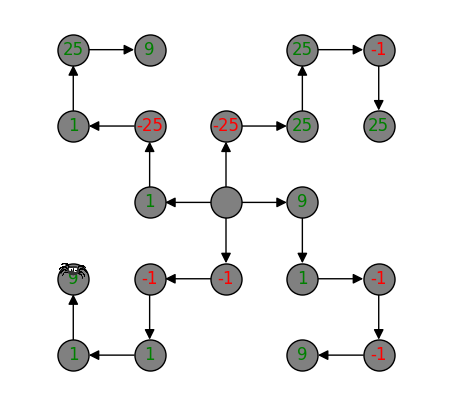
\includegraphics[width=0.6\linewidth]{image1.png}
    \caption{Illustration of the constant-variance environment used in our extension of Experiment 2. Each node conceals a reward (green or red), sampled from a common distribution (e.g.\ $\pm 25, \pm 9, \pm 1$). This figure is a schematic; actual experiments randomize the location of each reward at the start of each trial.}
    \label{fig:constant_env}
\end{figure}

As in Callaway et al.\ (2023), the rationale behind this manipulation is to examine whether human planners stick to a single search strategy (as one might expect from a purely best-first approach) or adapt to factors such as perceived risk, subjective cost, or time pressure. Our data collection modifies the original task to incorporate \emph{cognitive control} variables (e.g., self-reported workload, time intervals between clicks) that might modulate planning depth and direction. In particular, we ask:

\begin{itemize}
    \item \textbf{Adaptation of heuristics.} Do participants still gravitate toward a best-first approach in a constant reward setting, or can we observe variations when costs are high?
    \item \textbf{RL-based modeling.} Can a higher-level RL policy capture changes in the number of expansions, reflecting a real-time trade-off between exploration (revealing more nodes) and exploitation (terminating earlier to avoid cognitive costs)?
    \item \textbf{Outcome vs.\ effort.} How does the uniform risk across all states influence participants’ willingness to explore multiple paths? Do changes in subjective cost or time constraints lead to more rapid stopping?
\end{itemize}

Together, these questions extend the original Experiment 2 design to clarify how humans allocate cognitive resources even in “uniformly uncertain” environments. Our preliminary evidence suggests that although best-first expansions remain common, participants do \emph{adapt} when certain cost parameters (e.g., mental effort, time penalty) become sufficiently salient. Thus, consistent with the broader findings of Experiment 2, people adjust not only to the external environment but also to their own internal constraints and preferences.

\subsection*{Control Deprivation Manipulation and the Rationale for an RL Approach}

In addition to investigating resource-constrained planning, our study introduced an experimental manipulation designed to induce a sense of \emph{control deprivation} among participants. Specifically, we adopted a common psychological procedure in which participants were asked to complete a series of computer-based quiz tasks of varying durations (e.g., a shorter vs.\ a longer time allotment). After submitting their responses, participants received feedback about the correctness of their answers. Crucially, in the “deprivation” condition, this feedback was intentionally \emph{inaccurate}: although participants might have selected the correct response, we sometimes informed them that their response was wrong. Such false or discouraging feedback aims to diminish participants’ perceived efficacy and thus heighten their sense of frustration or lack of control.

Our motivation for incorporating this control-deprivation manipulation stems from the hypothesis that an individual’s feeling of control can significantly influence their decision-making processes, especially under constraints of time or cognitive resources. By varying both the time available (long vs.\ short quiz) and the accuracy of performance feedback, we sought to create a gradient of experienced control—ranging from a relatively empowered state to a distinctly deprived one. This gradient offers a window into how participants might shift their planning strategies and computational resource allocation when they perceive themselves as less or more in control of the situation.

\paragraph{Why Reinforcement Learning?}
We believe that modeling human decision-making in these scenarios using a \emph{Reinforcement Learning} (RL) framework provides important benefits over purely normative or heuristic-based models. In particular:
\begin{itemize}
    \item \textbf{Dynamic Adaptation:} RL models can track how participants adaptively tune their exploration and exploitation behaviors over multiple trials, especially under changing conditions of perceived control or feedback accuracy.
    \item \textbf{Cost--Benefit Analysis:} By framing each planning or search step as an action that incurs a cognitive or temporal cost, RL approaches naturally capture the trade-offs participants face. This aligns well with metalevel MDP perspectives, in which each computational step (e.g., expanding a node) is treated as a resource-intensive operation whose value must outweigh its cost.
    \item \textbf{Robustness to Noisy Feedback:} Because RL algorithms typically learn from observed rewards (and punishments) even if these signals are imperfect or stochastic, they are well-suited to modeling conditions where participants receive misleading or manipulative feedback. The agent’s policy evolves based on cumulative experience, mirroring the way real-world decision-makers gradually adjust strategy under uncertain or biased information.
\end{itemize}

Thus, by applying an RL-based modeling strategy to our control-deprivation design, we aim to gain deeper insights into how individuals reconfigure their planning or metacognitive policies in response to altered perceptions of control. In particular, we can assess whether participants’ sense of learned helplessness or heightened vigilance (due to false feedback) leads them to reduce their search depth, shift to simpler heuristic expansions, or otherwise deviate from rational metareasoning predictions. Our preliminary findings suggest that RL models capture these adaptive shifts more accurately than static or purely normative accounts, reinforcing the view that human planning should be studied as an ongoing, feedback-driven process. 

\section*{Methodology}
\subsection*{Overview of the Extended Mouselab-MDP Task}
We adopt a Mouselab-MDP style interface that externalizes planning operations by requiring participants to “click” on hidden rewards to reveal them. Under constant variance, each hidden reward $R_i$ follows an identical distribution, but participants incur a small time or point cost for each click. Unlike the original design, we incorporate self-reported workload ratings (via brief questionnaires) to gauge individual differences in perceived planning cost.

\subsection*{Cognitive Control Modeling}
\label{sec:cogcontrol}
We embed a \emph{cognitive control} parameter $\alpha$ in the metalevel reward function to reflect each individual’s sensitivity to planning costs. For instance, each node expansion might incur a cost $c(\alpha)$, which scales based on reported mental effort. This approach aligns with the notion that planning cost is subjective and context-dependent.  
We hypothesize that participants with higher $\alpha$ values exhibit shallower expansions (or switch to simpler heuristics earlier), whereas those with lower $\alpha$ might search more extensively. By fitting these models to participants’ revealed sequences, we aim to test whether a single parameter can explain large inter-individual differences in planning strategies.

\subsection*{Reinforcement Learning Perspective}
To tackle the combinatorial explosion of metalevel states, we use a reinforcement learning approach to approximate the optimal policy:
\begin{enumerate}
    \item \textbf{State Representation:} Encodes which nodes are revealed, partial reward estimates, and an internal memory of expansions.
    \item \textbf{Action Space:} Select a node to expand, or terminate and execute the best path found so far.
    \item \textbf{Reward Function:} Reflects the net external reward minus cost of expansions, factoring in $\alpha$ to capture personal effort.
    \item \textbf{Learning Algorithm:} A neural network approximator for $Q(\text{state}, \text{action})$ or a policy gradient method (e.g., PPO) to learn how to allocate expansions efficiently.
\end{enumerate}
\sloppy
\section*{Results and Analysis}

\subsection*{Impact of Control Deprivation on Planning Performance}

\begin{figure}[h]
    \centering
    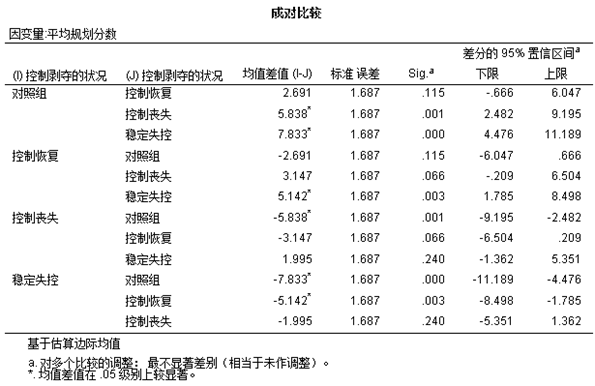
\includegraphics[width=0.8\linewidth]{image5.png}
    \caption{Post-hoc pairwise comparisons of mean planning scores}
    \label{fig:table_of_hoc}
\end{figure}
We conducted an analysis of variance (ANOVA) with the control deprivation condition as a between-subjects factor. The results indicate a significant main effect of control deprivation, 
\(F = -8.347,\; p = 0.000,\; \eta_p^2 = 0.239.\)
No significant interaction effect was found between the \emph{stability} of deprivation and the \emph{duration} of deprivation, suggesting that participants’ performance was primarily influenced by the overall status of their perceived control rather than how long or how stably it was removed.

\paragraph{Post-hoc pairwise comparisons.}
Using post-hoc tests to compare each condition:
\begin{itemize}
    \item \textbf{Control vs.\ Stable Control Deprivation.} The control group performed significantly better than the stable deprivation group (\(t=7.833, p=0.000,\; 95\%\ \mathrm{CI}=[4.476,\,11.189]\)).
    \item \textbf{Control vs.\ Loss of Control.} The control group also outperformed the loss-of-control group (\(t=5.838, p=0.001,\; 95\%\ \mathrm{CI}=[2.482,\,9.195]\)).
    \item \textbf{Recovery vs.\ Stable Control Deprivation.} Participants who experienced recovery performed significantly better than those with stable deprivation (\(t=5.142, p=0.003,\; 95\%\ \mathrm{CI}=[1.785,\,8.498]\)).
\end{itemize}

From these results, it is clear that removing or reducing participants’ sense of control leads to reliably lower planning scores relative to the control group. Notably, however, the analyses revealed no significant difference in another key measure (***), implying that the basic decision-making process might be fundamentally similar across groups. Consequently, we can apply the same RL-based model to each subset of participants’ data, allowing parameter estimates (e.g., cost or exploration parameters) to capture individual or subgroup differences without needing entirely separate model structures.

We evaluated four different models---\textsc{Breadth}, \textsc{Depth}, \textsc{Best}, and \textsc{Optimal}---alongside the aggregate \textsc{Human} data, focusing on how well each model fits participants’ decisions under our RL-based framework. Below, we present both quantitative (\emph{NLL}, \emph{AIC}, and \emph{GML}) and qualitative (behavioral curves) comparisons. 

\subsection*{Model Fit Using Geometric Mean Likelihood (GML)}
\label{sec:gml}
To gauge how closely each model’s policy predictions align with observed choices, we computed the negative log-likelihood (\(\mathrm{NLL}\)) for each trial and then derived the \textit{geometric mean likelihood} (\(\mathrm{GML}\)). For a total of \(\mathrm{N\_ACT}\) actions (clicks) and a sum of test negative log-likelihood \(\sum \mathrm{Test\_NLL}\), the average \(\overline{\mathrm{NLL}}\) is:
\[
  \overline{\mathrm{NLL}} \;=\; \frac{\sum \mathrm{Test\_NLL}}{\mathrm{N\_ACT}},
\]
and we define
\[
  \mathrm{GML} \;=\; \exp\bigl(-\,\overline{\mathrm{NLL}}\bigr).
\]
A higher GML indicates that the model yields higher likelihood for the human data.

\begin{table}[h]
    \centering
    \begin{tabular}{lcccc}
    \toprule
    \textbf{Model}
      & \(\sum \mathrm{Test\_NLL}\) 
      & \(\overline{\mathrm{NLL}}\) 
      & \(\mathrm{GML}\) \\
    \midrule
    \textsc{Breadth} & 16760.16 & 1.713 & 0.180 \\
    \textsc{Depth}   & 16012.89 & 1.637 & 0.195 \\
    \textsc{Best}    & 13492.14 & 1.379 & 0.252 \\
    \textsc{Optimal} & 12347.41 & 1.262 & 0.283 \\
    \bottomrule
    \end{tabular}
    \caption{Geometric Mean Likelihood (GML) for Different Models. Higher GML suggests a better fit to human data.}
    \label{tab:gml}
\end{table}

Figure~\ref{fig:gml_plot} visualizes these GML values. We see that \textsc{Optimal} attains the highest score, followed by \textsc{Best}, \textsc{Depth}, and \textsc{Breadth}.

\begin{figure}[h]
    \centering
    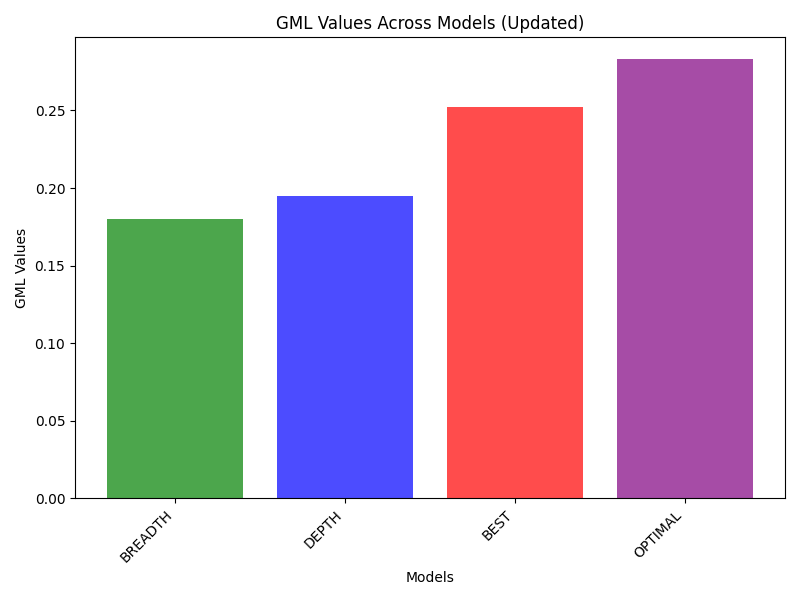
\includegraphics[width=0.6\linewidth]{image4.png}
    \caption{GML values across models. \textsc{Optimal} obtains the highest geometric mean likelihood, indicating it better captures participants' observed decisions compared to the other strategies.}
    \label{fig:gml_plot}
\end{figure}

\subsection*{Comparison of Strategy Curves}
We next compared how each model’s policy accumulates reward as the number of expansions (clicks) increases, and how it adjusts the second-click decision based on the first revealed value. Figures~\ref{fig:reward_vs_clicks} and \ref{fig:second_click} illustrate these trends:

\begin{enumerate}
    \item \textbf{Expected Reward vs.\ Number of Clicks} (Figure~\ref{fig:reward_vs_clicks}): 
    \textsc{Optimal} and \textsc{Best} generally track human performance more closely over a range of click counts, whereas \textsc{Breadth} lags behind until many nodes are revealed. \textsc{Depth} initially escalates more quickly than \textsc{Breadth} but still fails to match the final performance of \textsc{Best} and \textsc{Optimal}.

    \item \textbf{Proportion of Second Clicks on the Same Path} (Figure~\ref{fig:second_click}):
    We grouped trials by the value revealed on the first click and measured how often a second click remains on the same path. A strong dependence on the revealed value indicates a \emph{best-first} tendency, while a uniform pattern suggests \emph{breadth-first} or \emph{depth-first} expansions. In the human data (black dots), we observe a steep increase in same-path exploration for higher initial values, echoing \textsc{Best} and \textsc{Optimal} more closely than \textsc{Breadth} or \textsc{Depth}.
\end{enumerate}

\begin{figure}[h]
    \centering
    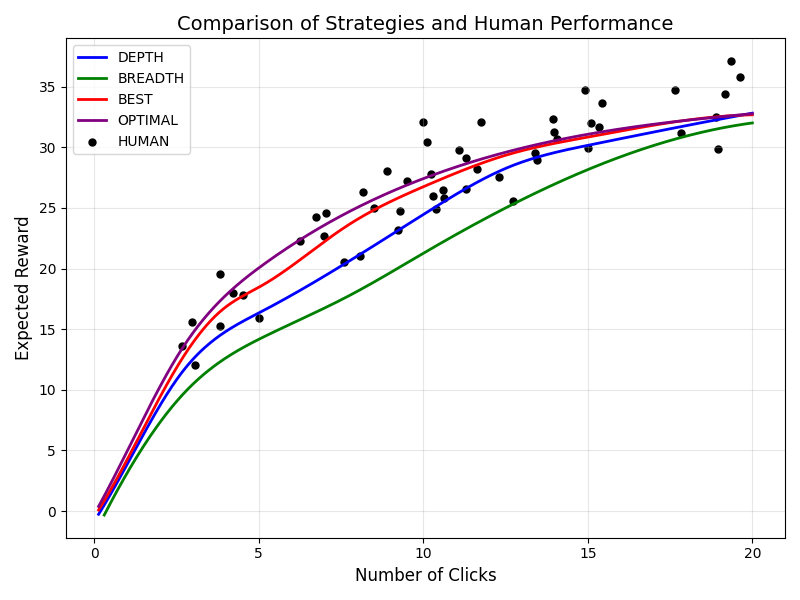
\includegraphics[width=0.6\linewidth]{image2.png}
    \caption{Comparison of Strategies and Human Performance. Each curve shows expected reward as a function of how many nodes the agent expands (clicks). Black dots indicate human participants’ aggregated data.}
    \label{fig:reward_vs_clicks}
\end{figure}

\begin{figure}[h]
    \centering
    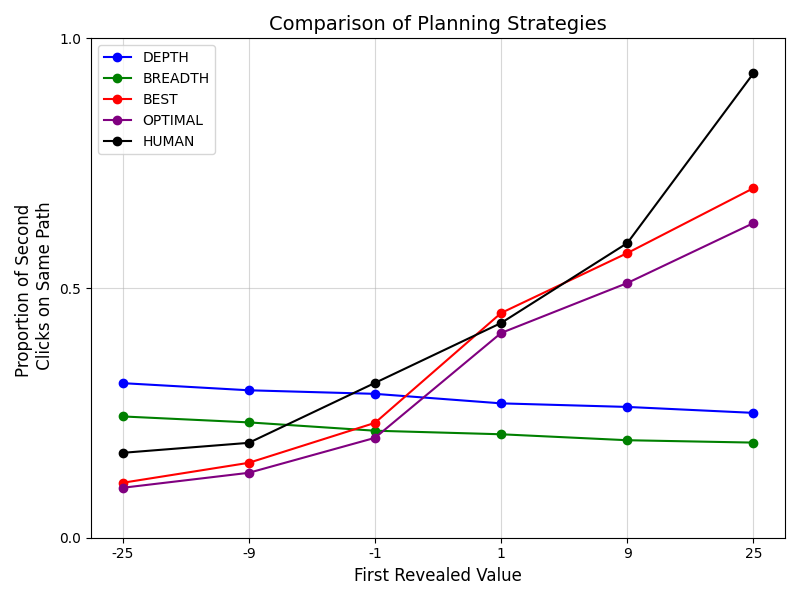
\includegraphics[width=0.6\linewidth]{image3.png}
    \caption{Proportion of second-click expansions on the same path as a function of the first revealed node's value. Human data (black) reveals a strong “best-first” tendency for high positive values, closely resembling the \textsc{Optimal} and \textsc{Best} curves.}
    \label{fig:second_click}
\end{figure}

\subsection*{AIC Computation and Model Ranking}
To further distinguish among models, we computed Akaike’s Information Criterion (AIC), which penalizes model complexity in addition to raw likelihood. Let \(\theta\) denote a model’s parameter vector of dimension \(k\). For data \(\{(x_i,\,y_i)\}_{i=1}^n\), we define
\[
\mathrm{NLL}(\theta)
=
- \sum_{i=1}^n 
  \ln \bigl[
    f\bigl(y_i \mid x_i,\;\theta\bigr)
  \bigr].
\]
The AIC is then
\[
\mathrm{AIC} \;=\; 2\,k + 2\,\mathrm{NLL}(\hat{\theta}),
\]
where \(\hat{\theta}\) is the MLE parameter estimate. Table~\ref{tab:AIC} shows the AIC scores and the resulting Akaike weights. \textsc{Optimal} emerges as the best-fitting model according to AIC, with a much lower score relative to the other approaches.

\begin{table}[h]
    \centering
    \begin{tabular}{lcccccc}
    \toprule
    \textbf{Model}
      & \(\textbf{k}\) 
      & \(\sum \mathrm{Test\_NLL}\)
      & \textbf{AIC}
      & \(\Delta_i\)
      & \(\exp(-\Delta_i/2)\)
      & \textbf{Akaike Weight}\\
    \midrule
    \textsc{Breadth}
      & 3
      & 16760.16
      & 33526.32
      & 8823.50
      & \(\approx 0.0\)
      & \(\approx 0.0\)\\
    \textsc{Depth}
      & 3
      & 16012.89
      & 32031.78
      & 7328.96
      & \(\approx 0.0\)
      & \(\approx 0.0\)\\
    \textsc{Best}
      & 3
      & 13492.14
      & 26990.28
      & 2287.46
      & \(\approx 0.0\)
      & \(\approx 0.0\)\\
    \textsc{Optimal}
      & 4
      & 12347.41
      & 24702.82
      & 0
      & 1.0
      & 1.0 \\
    \bottomrule
    \end{tabular}
    \caption{AIC Computation and Akaike Weights. \textsc{Optimal} dominates in terms of both AIC and associated weight.}
    \label{tab:AIC}
\end{table}

\subsection*{Discussion of Findings}
Collectively, these results suggest that while heuristic models (\textsc{Breadth}, \textsc{Depth}, \textsc{Best}) can approximate partial aspects of human behavior, the \textsc{Optimal} model provides a substantially better fit overall. This advantage is evident in terms of negative log-likelihood (reflected in higher GML) and penalized likelihood measures (AIC). Qualitative comparisons of how quickly each model escalates reward and how it reacts to initial high or low values further confirm that people’s strategy is closer to \textsc{Optimal} under this RL-based framework, at least within the “constant variance” environment we tested.

Moreover, the strong performance of \textsc{Optimal} highlights that human participants appear sensitive to both reward magnitudes and the cost of information. When large negative or positive outcomes are revealed, participants are more likely to adopt or abandon that path accordingly, mirroring the best-first component within \textsc{Optimal}.

In summary, consistent with \cite{Callaway2023rationaluse}, human planning in this environment shows adaptive patterns that neither purely match a single heuristic nor deviate so randomly as to suggest no systematic structure. Our extensions further indicate that an RL-based perspective, where planning itself is treated as a sequential decision problem, can help unify these results by modeling how participants dynamically balance exploration cost and potential reward.

\section*{Discussion and Ongoing Work}
By extending the constant variance condition of Callaway et al. (2023), we provide new evidence that individuals’ planning processes exhibit varying degrees of \emph{cognitive control} and can be partially captured by a metalevel MDP-based RL framework. This aligns with prior claims that planning is itself a sequential decision problem, with computations as actions and belief states as internal representations.  
Our approach further suggests that human resource allocation in planning can be systematically studied through the lens of RL, bridging cognitive psychology and AI research. One open question is how best to incorporate hierarchical RL for more complex tasks, in which subproblems can themselves be decomposed into smaller metalevel tasks. Another direction is to incorporate real-time psychophysiological or neural measures to refine $\alpha$ estimates and further validate the notion of cognitively controlled expansions.

\section*{Conclusion}
We have introduced an extended metalevel MDP model of resource-constrained planning, grounded in the “constant variance” setting of Experiment 2 in \cite{Callaway2023rationaluse} and enriched by a cognitive control component. Our collaboration with psychology researchers allowed us to integrate subjective workload into the metalevel cost function, offering a more nuanced view of how people decide when and where to invest mental effort. Additionally, we demonstrated how Reinforcement Learning techniques can be employed to approximate the metalevel policy for planning, emphasizing that planning itself is a sequential decision-making process at a higher level.  
Future work includes validating our cognitively controlled model across broader task domains, scaling up the RL framework to handle even more complex or high-dimensional planning problems, and exploring richer forms of individual differences in metacognitive awareness. We hope this research helps bridge the gap between cognitive modeling and practical AI systems that must allocate their limited computational resources adaptively.

\begin{thebibliography}{9}

\bibitem{Callaway2023rationaluse}
F. Callaway, B. van Opheusdena, S. Gulb, P. Dasc, P. Kruegerd, T. L. Griffithsa,d, and F. Liedere,
\newblock ``Rational use of cognitive resources in human planning,''
\newblock \textit{Proceedings of the National Academy of Sciences}, 2023.

\bibitem{griffiths2015rational}
T. L. Griffiths, F. Lieder, and N. D. Goodman,
\newblock ``Rational use of cognitive resources: Levels of analysis between the computational and the algorithmic,''
\newblock \textit{Topics in Cognitive Science}, vol. 7, no. 2, pp. 217--229, 2015.

\bibitem{payne1993adaptive}
J. W. Payne, J. R. Bettman, and E. J. Johnson,
\newblock \textit{The Adaptive Decision Maker},
\newblock Cambridge University Press, 1993.

\bibitem{sutton2018reinforcement}
R. S. Sutton and A. G. Barto,
\newblock \textit{Reinforcement Learning: An Introduction},
\newblock MIT Press, 2nd edition, 2018.

\end{thebibliography}

\end{document}
